\documentclass[12pt,a4paper]{article}
\usepackage{hw}

\graphicspath{ {.} }
\begin{document}
\qtitle{8.1}
For t-distribution, $t=(\overline{X}-\mu)/(s/\sqrt{N})$. Simliar to equation 8.7, \\ 
$x_t=x_{1-\alpha}=x_{\beta}=\cfrac{s}{\sqrt{N}}z_{1-\alpha}+\mu=\cfrac{s}{\sqrt{N}}z_{\beta}+\mu+d$, then
\begin{equation}
N=\cfrac{s^2}{d^2}(t_{1-\alpha}+t_{1-\beta})^2
\end{equation}

\noindent Since $s^2$ has $N-1$ degrees of freedom. When $N$ is large (eg: $>20$), $s\rightarrow \sigma$. As example 8.2.4 said, $detectability=\cfrac{d}{\sigma}\approx\cfrac{d}{s}=0.5$. 

\textbf{a)}. For $\alpha=\beta=0.05$, from normal distribution $z$ in the example, we assume $N_a=44$ and $t_{1-\alpha}=t_{1-\beta}=t_{0.95}=tinv(0.95,44-1)=1.681$, which is slightly larger than $z_{1-\beta}=1.645$. \\
According to (1), $N=4(2*1.681)^2=45\ne N_a$. The presumed sample size to compute t doesn't match the output, perhaps nuance between $s^2$ and $\sigma^2$ is also one of the reasons. So we try $N_a=45$, $t_{0.95,44}=1.680$, then $N\approx45=N_a$. Therefore, minimum sample size $N=45$ may be the better option when changing from  $z$ to $t$.

\textbf{b)}. Likewise, for $\alpha=\beta=0.01$, as the example illustrated, we assume $N_a=87$, then $t_{0.99,86}=tinv(0.99,87-1)=2.37$. According to (1), $N=4(2*2.37)^2\approx90\ne N_a$. So we try $N_a=90$, $N\approx90=N_a$. In this case, the minimum sample size should be 90.

As we can see, when changing from $z$ to $t$, the minimum sample size increases. If the type I and type II error need to be further reduced, the increasement degree would be even larger. This indicates the normal distribution is more condensed than t-distribution, especially in the tail region. 

\newpage
\qtitle{8.2}
\textbf{a.} Since $PPV=Pr(W|P)\\=\cfrac{Pr(P|W)Pr(W)}{Pr(P)}=\cfrac{Pr(P|W)Pr(W)}{Pr(P|W)Pr(W)+Pr(P|W^c)Pr(W^c)}$

\noindent For A, $PPV_A=\cfrac{0.9*0.5}{0.9*0.5+(1-0.99)*(1-0.5)}=0.989$\\
For B, $PPV_B=\cfrac{0.99*0.5}{0.99*0.5+(1-0.9)*(1-0.5)}=0.908$\\
So test A has best PPV.

\noindent \textbf{b.} When Prevalence is 0.01, then \\
$PPV_A=\cfrac{0.9*0.01}{0.9*0.01+(1-0.99)*(1-0.01)}=0.476\\
PPV_B=\cfrac{0.99*0.01}{0.99*0.01+(1-0.9)*(1-0.01)}=0.09$\\
So $PPV_A>>PPV_B$. To achieve high PPV, the specificity (TNF) should be low enough, especially when prevalence is small. When prevalence is small, low specificity would cause large number of false positive tests because the normal population is much larger. 

\newpage
\qtitle{8.3}
\textbf{a.} Convert $\overline x$ to $z$, $z=\cfrac{\overline x-\mu}{\sigma / \sqrt(N)}$. For $N=10,30,50$, we would get the following distributions (shown in histograms).
\begin{figure}[!ht]
    \centering
    \includegraphics*[width=\textwidth]{hw_8_3_dist.png}
    \caption{Histogram of z value distributions}
\end{figure} 

Corresponding ROC figures are:
\begin{figure}[!ht]
    \centering
    \includegraphics*[width=\textwidth]{hw_8_3_roc.png}
\end{figure}

Their AUCs are 0.61, 0.83, and 0.93 respectively. The AUC increases with N increases. This is because the sample size increases with $N^2$ fold. As shown in Figure 8.1, as separability $d\sqrt{N}/\sigma$between $g_0$ and $g_1$ increases with $\sqrt{N^2}=N$ fold. Therefore, since AUC increases as the separability increases, the $N=50$ would achieve largest AUC value. But the increasement is non-linear. 

Code to get FPF and TPF:
\begin{lstlisting}
...
[N0,E0] = histcounts(g0_mean_z, "Normalization", 'probability');
[N1,E1] = histcounts(g1_mean_z, "Normalization", 'probability');
...
count = 1;
fpf = zeros(length(E0),1);
tpf = zeros(length(E0),1);
for t=E0
    fpf(count) = sum(N0(count:end));
    id = find(abs(E1-t)<1e-4);
    if isempty(id) 
        tpf(count)=sum(N1);
    else
        tpf(count)=sum(N1(id:end));
    end
    count = count+1;
end
\end{lstlisting}

\vspace{0.5cm}
\textbf{b.} 
$b_i-a_i$ increases from 10 to 20, so the variance increases due to the data is less condensed. The separability $d\sqrt{N}/(\sigma)$ decreases as the variance increases. It means that the AUC would decrease. In detail, it drops from 0.95 to 0.73.  
\begin{figure}[!ht]
    \centering
    \includegraphics*[width=\textwidth]{hw_8_3_b.png}
\end{figure}

\vspace{0.5cm}
\textbf{c.}
$d'=d\sqrt{N}/\sigma$ and $d_a=2erf^{-1}(2AUC-1)$

\noindent 1). For $b_i-a_i=10$ in \textbf{a}, $\sigma=\sqrt{5.33}, d=0.1\rightarrow$\\
For $N=10$, $d'=0.1*\sqrt{10*10}/\sqrt{5.33}=0.433; d_a=2erf^{-1}(2*0.61-1)=0.395$\\
For $N=30$, $d'=1.299;d_a=1.349$\\
For $N=50$, $d'=2.166;d_a=2.08$

\vspace{0.5cm}
\noindent 2). For $b_i-a_i=20$ in \textbf{b}, $\sigma=\sqrt{33.3},d=0.1,AUC_10=0.55,AUC_30=0.64;AUC_50=0.73\rightarrow$\\
For $N=10$, $d'=0.173;d_a=0.178$\\
For $N=30$, $d'=0.52;d_a=0.507$\\
For $N=50$, $d'=0.866;d_a=0.866$

Now we can see that $d'$ is very close to $d_a$. Also, when variance is larger, the their discrepancy is smaller.

\vspace{0.5cm}
\textbf{d.}
To achieve minimum total error, that is to minimize $\alpha+\beta$. As shown in the following figure, 
\begin{figure}[!ht]
\centering
\includegraphics*[width=\textwidth]{hw_8_3_d.png}
\caption{The blue line indicates $\alpha+\beta$ total error along z values.}
\end{figure}

To achieve the minimum total error, we should select z where the overlap of $g_0$ and $g_1$ distribution peaks. For \textbf{a}, the threshold on z axis should be 0.3, 0.6, 1.2 corresponding to N=10, 30, 50. Convert z to $\overline x$, $\overline x=\cfrac{\sigma}{\sqrt{N}}z+\mu$. Then the threshold on x axis should be 6.069, 6.023, 6.014.

Likeiwse, for $b$, $z=0,0,0.6\rightarrow \overline x=10,10,10.069$. But in this case, the AUC is low when N is small, the threshold doesn't make sense so much as in situation \textbf{a}.
Overall, the thresholds all cluster around mean value, since the separability is quite small in this problem. 

\newpage
\qtitle{8.4}
\textbf{1).} In example 8.3.1, $Z_0$ and $Z_1$ is standard normal distribution. Let $\sigma_0=2\sigma_1 \rightarrow \sigma_0=1;\sigma_1=0.5$, then change the 1 in the following lines into 0.5:
\begin{lstlisting}
...
Z1(j,:)=normpdf(z,d(j),1)
...
FP(j,Nz-k+1)=cdf('norm',z(k),0,1,'upper');
...
\end{lstlisting}  

\begin{figure}[!ht]
\centering
\includegraphics*[width=\textwidth]{hw_8_4_a.png}
\caption{$\sigma_0=2\sigma_1$. Left figure shows pdfs (the shorter one centering at 0 is $Z_0$, the rest are $Z_1$); the middle shows the ROC curves; the right shows the AUCs. The blue dotted line is the AUC curve when $\sigma_0=\sigma_1$}
\end{figure}

\textbf{2).} Likewise, Let $\sigma_1=2$,
\begin{figure}[!ht]
    \centering
    \includegraphics*[width=\textwidth]{hw_8_4_b.png}
    \caption{$\sigma_0=2\sigma_1$. Left figure shows pdfs (the taller one centering at 0 is $Z_0$, the rest are $Z_1$); the middle shows the ROC curves; the right shows the AUCs. The blue dotted line is the AUC curve when $\sigma_0=\sigma_1$}
\end{figure}

Base on the tail part shown in the follwoing figure, tail is heavier when $\sigma$ is larger, which means pdf is less condensed.

If variances are unequal and $\sigma_0>\sigma_1$, when the threshold moves from right to left along axis from 3 to 1, FPF $\alpha$ starts increasing and FPF $1-\beta$ is still around 0; when from 1 to -1, TPF's increasement is much larger than FPF; when threshold is less than -1; TPF is almost 1 while FPF could still reduce. Therefore, the ROC curves are in convex sigmoid shape and AUCs are larger. 

If $\sigma_0<\sigma_1$, on the contrary, the ROC curves would be in concave sigmoid shape and AUCs are smaller. 

\begin{figure}[!ht]
\centering
\includegraphics*[width=0.6\textwidth]{hw_8_4_sigma.png}
\caption{pdfs when $\sigma=1,0.5,2$ (cyan, blue, red curve)}
\end{figure}

\newpage
\qtitle{8.5}
\textbf{a.} $N=10\Rightarrow t_{0.025,9}=-t_{0.975,9}=tinv(0.025,9)=2.262$. So the 95\% CI is: $t_{0.025,9}<\cfrac{\overline X-\mu}{s/\sqrt{N}}<t_{0.975,9}\Rightarrow
-2.262*s/3<\overline X-\mu<2.262*s/3\\\Rightarrow\mu-0.754s<\overline X <\mu+0.754s$. Since $\mathcal{E}s^2=\sigma^2$, so 95\% CI bounds for mean cholesterol is:\\ $\mu\pm 0.754s\approx\mu\pm 0.754\sigma\rightarrow[220-0.754*20,220+0.754*20]=[204.9,235.1]$

\noindent\textbf{b.} If population standard variance $s$ is known, the CI range is ensured with length $2*0.754s=1.508s$, though the center of CI still could jitter around population mean. Compared with CIs in \textbf{a}, $s$ is unbiased which jitters around $\sigma$. So the CIs would change little when population standard deviation is known.   

\noindent\textbf{c.} 
Using following code to conduct 10 experiements:
\begin{lstlisting}
samp=10;exp=10;
g0=normrnd(220,20,[samp,1,exp]);
% ci_l = mean(g0, 'all')-0.754*sqrt(var(g0,0,'all'));
% ci_h = mean(g0, 'all')+0.754*sqrt(var(g0,0,'all'));
ci_l = 204.9;ci_h=235.1;
g0_mean = zeros(exp,1);
for i=1:exp
    g0_mean(i) = mean(g0(:,:,i), 'all');
end
match_count = sum((ci_l < g0_mean) & (g0_mean< ci_h));
disp(match_count)
\end{lstlisting}
The sample mean of each experiment falls in the CI.
\begin{figure}[!ht]
    \centering
    \includegraphics*[width=0.6\textwidth]{hw_8_5_ci.png}
    \caption{blue circles are sample means; red circles are CI bounds.}
\end{figure}

When conducting such experiment for 10 trials, we see almost all sample means would fall in this interval. 
\begin{figure}[!ht]
\centering
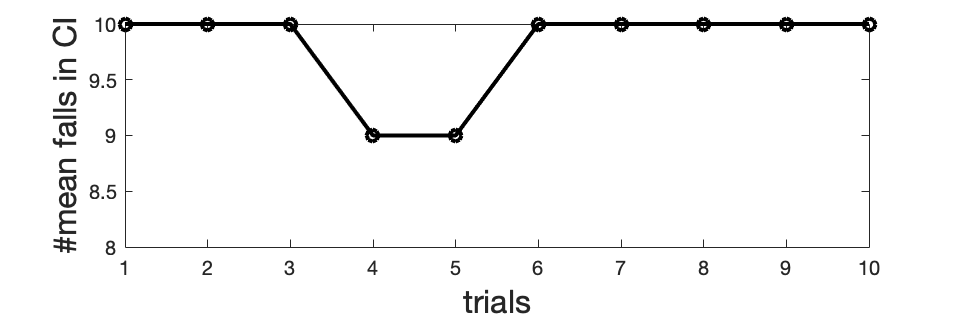
\includegraphics[width=0.5\textwidth]{hw_8_5.png}
\end{figure}

\end{document}
